% mGFS Design, Implementation & Testing Report
\documentclass[10pt,a4paper]{article}

\usepackage[UTF8]{ctex}
\usepackage{geometry}
\usepackage{graphicx}
\usepackage{tikz}
\usepackage{listings}
\usepackage{xcolor}
\usepackage{booktabs}
\usepackage{tabularx}
\usepackage{hyperref}
\usepackage{float}
\usepackage{enumitem}
\usepackage{fancyhdr}
\usepackage{caption}

\usetikzlibrary{arrows, arrows.meta, shapes, shapes.geometric, positioning,
                fit, calc, backgrounds}

\geometry{left=2.5cm, right=2.5cm, top=3cm, bottom=3cm}

% \pagestyle{fancy}
% \fancyhf{}
% \rhead{mGFS 分布式文件系统}
% \lhead{云计算与虚拟化技术}
\cfoot{\thepage}

\definecolor{codebg}{RGB}{248,248,248}
\definecolor{codeframe}{RGB}{200,200,200}
\definecolor{kw}{RGB}{0,0,180}
\definecolor{str}{RGB}{163,21,21}
\definecolor{cmt}{RGB}{0,128,0}

\lstset{
  backgroundcolor=\color{codebg},
  frame=single,
  rulecolor=\color{codeframe},
  basicstyle=\ttfamily\small,
  keywordstyle=\color{kw}\bfseries,
  stringstyle=\color{str},
  commentstyle=\color{cmt}\itshape,
  breaklines=true,
  numbers=left,
  numberstyle=\tiny\color{gray},
  numbersep=5pt,
  tabsize=4,
  showstringspaces=false,
}

\hypersetup{colorlinks=true, linkcolor=blue!60!black, urlcolor=blue!60!black}

% ─────────────────────────────────────────────────────────────
\title{
  \vspace{-1cm}
  {\Large 云计算与虚拟化技术 \quad 作业五}\\[0.8em]
  {\huge \textbf{mGFS 分布式文件系统}}\\[0.4em]
  % {\large 设计、实现与测试报告}\\[1em]
  % \rule{\linewidth}{0.5pt}
}
\author{2351044 崔艺洋}
\date{\today}

\begin{document}
\maketitle
% \thispagestyle{empty}
\tableofcontents
\newpage

% ═══════════════════════════════════════════════════════════════
\section{项目概述}

mGFS（Mini Google File System）是基于 Google GFS 论文~\cite{gfs2003} 的简化 Python 实现，
采用 Apache Thrift 作为 RPC 框架，实现了 GFS 的核心机制：
单主节点元数据管理、64\,MB 分块存储、三副本写入与基于租约的主副本选举。

\subsection{核心设计目标}

\begin{itemize}[leftmargin=2em]
  \item \textbf{大文件分块}：以 64\,MB 为单位切分，支持任意偏移读写与追加。
  \item \textbf{多副本容错}：每块默认 3 副本；读操作自动故障转移至健康副本。
  \item \textbf{集中式元数据}：Master 唯一维护文件-块-位置映射，全部驻留内存。
  \item \textbf{租约一致性}：60\,s 基于时间的租约确定主副本，协调并发写入。
\end{itemize}

\subsection{技术栈}

\begin{table}[H]
\centering
\caption{技术栈}
\begin{tabularx}{\textwidth}{lX}
\toprule
\textbf{组件} & \textbf{选型} \\
\midrule
语言        & Python 3 \\
RPC 框架    & Apache Thrift（thriftpy2 动态加载 IDL）\\
并发模型    & \texttt{threading.Lock} + 守护线程 \\
配置格式    & XML（gfs-site.xml）\\
测试框架    & \texttt{unittest}（30 个用例）\\
\bottomrule
\end{tabularx}
\end{table}

% ═══════════════════════════════════════════════════════════════
\section{系统架构设计}

\subsection{整体架构}

mGFS 沿用 GFS 的三层架构：客户端（Client）、主节点（Master）和数据节点（ChunkServer）。
所有通信经由 Thrift RPC 完成，Master 与 ChunkServer 分别暴露独立服务接口，如图~\ref{fig:arch} 所示。

\begin{figure}[H]
\centering
\begin{tikzpicture}[
  node distance=1.4cm and 2.4cm,
  every node/.style={font=\small},
  box/.style={rectangle, rounded corners=4pt, draw, minimum width=2.8cm,
              minimum height=1cm, align=center},
  cs/.style ={box, fill=blue!12},
  ms/.style ={box, fill=orange!20},
  cl/.style ={box, fill=green!12},
  arr/.style={-{Stealth[scale=0.8]}, thick},
  darr/.style={<->, thick, dashed, gray},
]
\node[cl] (C)  {GFSClient};
\node[ms, right=4.6cm of C] (M)  {Master\\（Meta Data）};
\node[cs, above right=0.7cm and 1.2cm of M] (S1) {ChunkServer\\cs1\;:9091};
\node[cs, right=2.2cm of M]                  (S2) {ChunkServer\\cs2\;:9092};
\node[cs, below right=0.7cm and 1.2cm of M] (S3) {ChunkServer\\cs3\;:9093};

\draw[arr, bend left=15] (C) to node[pos=0.55, above,sloped]{\scriptsize MasterService}  (M);
\draw[arr, bend left=15] (M) to node[pos=0.4, below,sloped]{\scriptsize ChunkInfo/FileInfo} (C);

\draw[arr] (C.north east) to[bend left=20]
           node[pos=0.65, above,sloped]{\scriptsize ChunkService} (S1.west);
\draw[arr] (C.east) -- node[pos=0.25, above]{\scriptsize read/write} (S2.west);
\draw[arr] (C.south east) to[bend right=20]
           node[pos=0.65, below,sloped]{\scriptsize ChunkService} (S3.west);

\draw[darr] (M.north east) to[bend left=5]  node[above,sloped]{\scriptsize heartbeat} (S1.west);
\draw[darr] (M.east)        --               node[above]{\scriptsize heartbeat}        (S2.west);
\draw[darr] (M.south east) to[bend right=5] node[below,sloped]{\scriptsize heartbeat} (S3.west);
\end{tikzpicture}
\caption{mGFS 系统架构图}
\label{fig:arch}
\end{figure}

\subsection{RPC 接口（gfs.thrift）}

\begin{lstlisting}[language=Java, caption={Thrift IDL 核心定义}]
struct ChunkInfo {
    1: string chunk_handle,
    2: list<string> locations,
    3: string primary
}
struct FileInfo {
    1: string file_name,
    2: i64 file_size,
    3: list<string> chunk_handles
}
service MasterService {
    bool      create_file(1: string filename),
    bool      delete_file(1: string filename),
    FileInfo  get_file_info(1: string filename),
    ChunkInfo get_chunk_handle(1: string filename, 2: i32 chunk_index),
    bool      heartbeat(1: string server_id, 2: list<string> chunk_handles)
}
service ChunkService {
    string read(1: string chunk_handle, 2: i32 offset, 3: i32 length),
    bool   write(1: string chunk_handle, 2: i32 offset, 3: string data),
    bool   append(1: string chunk_handle, 2: string data),
    bool   copy_snapshot(1: string source, 2: string destination)
}
\end{lstlisting}

\subsection{元数据模型}

Master 在内存中维护两张核心映射表及一张租约表，关系如图~\ref{fig:meta} 所示。

\begin{figure}[H]
\centering
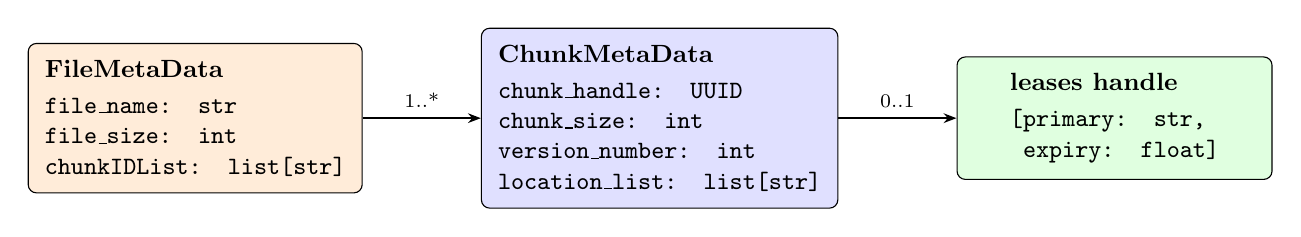
\begin{tikzpicture}[
  node distance=0.4cm and 1.8cm,
  every node/.style={font=\small},
  rec/.style={rectangle, draw, rounded corners=3pt, align=left,
              minimum width=4cm, inner sep=6pt},
  arr/.style={-{Stealth[scale=0.7]}, thick},
]
\node[rec, fill=orange!15] (FM) {
  \textbf{FileMetaData}\\[2pt]
  \texttt{file\_name: str}\\
  \texttt{file\_size: int}\\
  \texttt{chunkIDList: list[str]}
};
\node[rec, fill=blue!12, right=1.5cm of FM] (CM) {
  \textbf{ChunkMetaData}\\[2pt]
  \texttt{chunk\_handle: UUID}\\
  \texttt{chunk\_size: int}\\
  \texttt{version\_number: int}\\
  \texttt{location\_list: list[str]}
};
\node[rec, fill=green!12, right=1.5cm of CM] (LS) {
  \textbf{leases handle}\\[2pt]
  \texttt{[primary: str,}\\
  \texttt{\ expiry: float]}
};
\draw[arr] (FM.east) -- node[above]{\scriptsize 1..*} (CM.west);
\draw[arr] (CM.east) -- node[above]{\scriptsize 0..1} (LS.west);
\end{tikzpicture}
\caption{Master 内存元数据结构关系}
\label{fig:meta}
\end{figure}

% ═══════════════════════════════════════════════════════════════
\section{关键算法设计}

\subsection{分块分配}

当客户端首次访问某块时，Master 在持锁状态下：
（1）生成 \texttt{uuid4()} 作为全局唯一块句柄；
（2）从在线 ChunkServer 字典选取前 $\min(N,3)$ 个节点；
（3）写入 \texttt{ChunkMetaData}；
（4）调用租约模块确定主副本。

\subsection{租约与主副本选举}

\begin{figure}[H]
\centering
\begin{tikzpicture}[
  node distance=0.55cm and 0.2cm,
  every node/.style={font=\small},
  decision/.style={diamond, draw, fill=yellow!20, aspect=2.2, align=center,
                   inner sep=2pt},
  process/.style={rectangle, rounded corners=3pt, draw, fill=white,
                  minimum width=4.2cm, minimum height=0.8cm, align=center},
  startstop/.style={rounded rectangle, draw, fill=gray!15,
                    minimum height=0.7cm, align=center},
  arr/.style={-{Stealth[scale=0.7]}, thick},
]
\node[startstop] (s)  {\texttt{\_get\_or\_grant\_lease(chunk\_handle, locations)}};
\node[decision, below=0.7cm of s]  (d1) {租约存在?};
\node[decision, right=1.5cm of d1] (d2) {未过期\\且 primary 在线?};
\node[process, right=1.5cm of d2]  (p1) {续租 +60\,s\\返回现有 primary};
\node[process, below=1.4cm of d1]  (p2) {\texttt{locations[0]} 升为 primary\\写入新租约};
\node[startstop, below=0.7cm of p2](e)  {返回 primary};

\draw[arr] (s)  -- (d1);
\draw[arr] (d1) -- node[above]{\scriptsize 是} (d2);
\draw[arr] (d1) -- node[right]{\scriptsize 否} (p2);
\draw[arr] (d2) -- node[above]{\scriptsize 是} (p1);
\draw[arr] (d2) -- node[below]{\scriptsize 否} (p2);
\draw[arr] (p1.south) |- (e.east);
\draw[arr] (p2) -- (e);
\end{tikzpicture}
\caption{租约授予 / 续租流程}
\label{fig:lease}
\end{figure}

\subsection{写入流水线}

客户端通过 \texttt{DataQueue}（数据包缓冲）和 \texttt{ACKQueue}（确认追踪）
实现写入协议，流程如图~\ref{fig:write} 所示。

\begin{figure}[H]
\centering
\begin{tikzpicture}[
  node distance=0.55cm and 1.6cm,
  every node/.style={font=\small},
  stepbox/.style={rectangle, rounded corners=3pt, draw, fill=white,
               minimum width=5cm, minimum height=0.8cm, align=center},
  decision/.style={diamond, draw, fill=yellow!20, aspect=2.2, align=center,
                   inner sep=2pt},
  cs/.style={rectangle, draw, fill=blue!10, minimum width=2.8cm,
             minimum height=0.7cm, align=center},
  arr/.style={-{Stealth[scale=0.7]}, thick},
]
\node[stepbox] (p1) {创建 PacketMetaData（uuid packet\_id）};
\node[stepbox, below=of p1] (p2) {DataQueue.enqueue\\ACKQueue.expect(所有副本)};
\node[stepbox, below=of p2] (p3) {顺序调用 cs.write() 至每个副本};
\node[stepbox, below=of p3] (p4) {每成功返回 → ACKQueue.ack(packet\_id, server\_id)};
\node[decision, below=0.7cm of p4] (d) {ACKQueue\\is\_complete?};
\node[cs, right=1.5cm of d]  (ok) {成功返回};
\node[stepbox, left=1.5cm of d] (r)  {stream\_recovery\\（健康副本重试）};

\draw[arr] (p1)--(p2);  \draw[arr] (p2)--(p3);
\draw[arr] (p3)--(p4);  \draw[arr] (p4)--(d);
\draw[arr] (d) -- node[above]{\scriptsize 完整} (ok);
\draw[arr] (d) -- node[above]{\scriptsize 不完整} (r);

% ChunkServer nodes on the right
\node[cs, above right=0.3cm and 1.5cm of p3] (cs1) {cs1 (primary)};
\node[cs, right=1.5cm of p3]                  (cs2) {cs2};
\node[cs, below right=0.3cm and 1.5cm of p3] (cs3) {cs3};

\draw[-{Stealth[scale=0.6]}, dashed, gray] (p3.east) to[bend left=5]  (cs1.west);
\draw[-{Stealth[scale=0.6]}, dashed, gray] (p3.east) --                (cs2.west);
\draw[-{Stealth[scale=0.6]}, dashed, gray] (p3.east) to[bend right=5] (cs3.west);
\end{tikzpicture}
\caption{写入流水线流程图}
\label{fig:write}
\end{figure}

\subsection{读故障转移}

\texttt{\_read\_from\_replica} 按副本列表顺序逐一尝试，返回首个成功结果，
失败副本静默跳过：

\begin{lstlisting}[language=Python, caption={读故障转移核心逻辑（client.py）}]
def _read_from_replica(self, chunk_info, offset, length):
    for server_id in chunk_info.locations:
        try:
            host, port = self.chunk_server_ports[server_id]
            with make_client(ChunkService, host, port) as cs:
                return cs.read(chunk_info.chunk_handle, offset, length)
        except Exception:
            continue
    return ""
\end{lstlisting}

% ═══════════════════════════════════════════════════════════════
\section{系统实现}

\subsection{目录结构}

\begin{figure}[H]
\centering
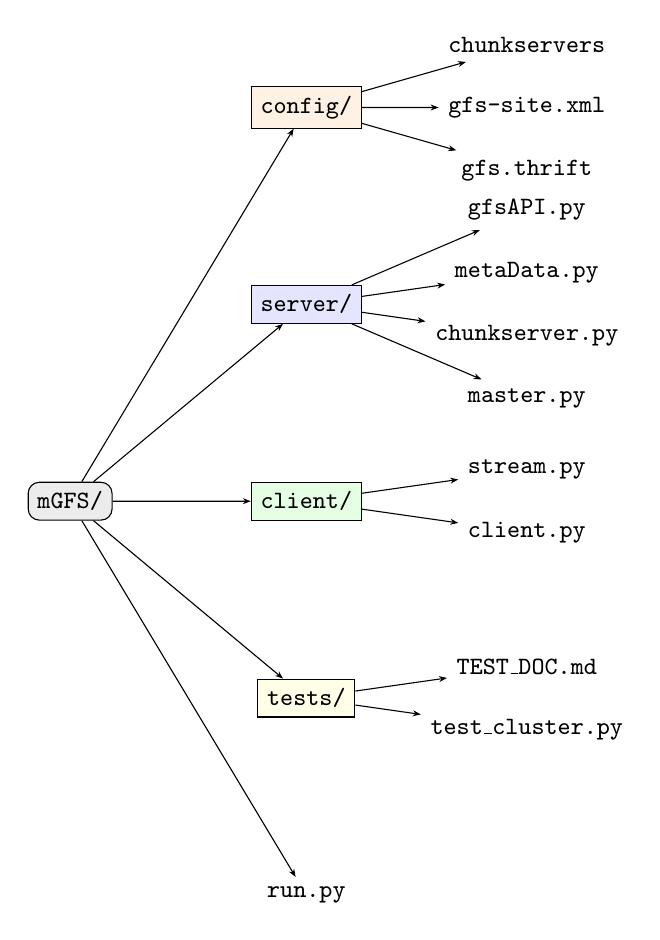
\begin{tikzpicture}[
  grow=right,
  every node/.style={font=\ttfamily\small},
  edge from parent/.style={draw, -{Stealth[scale=0.6]}},
  level 1/.style={sibling distance=2.5cm, level distance=3cm},
  level 2/.style={sibling distance=0.8cm, level distance=2.8cm},
]
\node[draw, rounded corners, fill=gray!15] {mGFS/}
  child { node {run.py} }
  child { node[draw,fill=yellow!10] {tests/}
    child { node {test\_cluster.py} }
    child { node {TEST\_DOC.md} }
  }
  child { node[draw,fill=green!10] {client/}
    child { node {client.py} }
    child { node {stream.py} }
  }
  child { node[draw,fill=blue!10] {server/}
    child { node {master.py} }
    child { node {chunkserver.py} }
    child { node {metaData.py} }
    child { node {gfsAPI.py} }
  }
  child { node[draw,fill=orange!10] {config/}
    child { node {gfs.thrift} }
    child { node {gfs-site.xml} }
    child { node {chunkservers} }
  };
\end{tikzpicture}
\caption{项目目录结构}
\label{fig:dir}
\end{figure}

\subsection{Master 节点状态}

\begin{table}[H]
\centering
\caption{Master 内部状态表（server/master.py）}
\begin{tabularx}{\textwidth}{llX}
\toprule
\textbf{属性} & \textbf{类型} & \textbf{用途} \\
\midrule
\texttt{file\_meta\_data}  & \texttt{dict[str, FileMetaData]}  & filename → 文件元数据 \\
\texttt{chunk\_meta\_data} & \texttt{dict[str, ChunkMetaData]} & handle → 块元数据 \\
\texttt{chunkservers}      & \texttt{dict[str, float]}         & server\_id → 最近心跳时间戳 \\
\texttt{leases}            & \texttt{dict[str, (str, float)]}  & handle → (primary, 到期时间) \\
\bottomrule
\end{tabularx}
\end{table}

\subsection{ChunkServer 块存储实现}

ChunkServer 以 \texttt{bytearray} 实现内存随机偏移写入，支持动态扩展：

\begin{lstlisting}[language=Python, caption={ChunkServer.write（server/chunkserver.py）}]
def write(self, chunk_handle, offset, data):
    with self.lock:
        encoded = data.encode('utf-8')
        if chunk_handle not in self.chunk_data:
            self.chunk_data[chunk_handle] = bytearray()
        buf = self.chunk_data[chunk_handle]
        end = offset + len(encoded)
        if len(buf) < end:
            buf.extend(b'\x00' * (end - len(buf)))  # zero-fill
        buf[offset:end] = encoded
        return True
\end{lstlisting}

\subsection{流水线抽象（client/stream.py）}

\begin{table}[H]
\centering
\caption{流水线原语类}
\begin{tabularx}{\textwidth}{lX}
\toprule
\textbf{类} & \textbf{职责} \\
\midrule
\texttt{DataQueue} & 线程安全 FIFO，缓存待发送的 \texttt{PacketMetaData}（enqueue/dequeue/peek）\\
\texttt{ACKQueue}  & 追踪每个 packet 期望的副本 ACK 集合；提供 \texttt{expect}/\texttt{ack}/\texttt{is\_complete} 等 \\
\bottomrule
\end{tabularx}
\end{table}

\subsection{配置参数（gfs-site.xml）}

\begin{table}[H]
\centering
\caption{集群配置参数默认值}
\begin{tabularx}{\textwidth}{llX}
\toprule
\textbf{键} & \textbf{默认值} & \textbf{说明} \\
\midrule
\texttt{gfs.master.port}         & 9090      & Master 监听端口 \\
\texttt{gfs.chunk.size}          & 67108864  & 块大小（64\,MB）\\
\texttt{gfs.replication}         & 3         & 副本数 \\
\texttt{gfs.lease.duration}      & 60        & 租约时长（秒）\\
\texttt{gfs.heartbeat.interval}  & 5         & 心跳间隔（秒）\\
\bottomrule
\end{tabularx}
\end{table}

% ═══════════════════════════════════════════════════════════════
\section{测试设计与结果}

\subsection{测试环境}

测试脚本（\texttt{test\_cluster.py}）在进程内以守护线程形式启动完整集群，
避免外部依赖：Master 端口 19090，ChunkServer 端口 19091--19093。

\subsection{测试用例分组}

\begin{figure}[H]
\centering
\begin{tikzpicture}[font=\small, every node/.style={font=\small}]
\foreach \i/\label/\cnt in {
  0/{T01--T03\quad 集群启动}/3,
  1/{T04--T09\quad 文件操作}/6,
  2/{T10--T13\quad 块分配}/4,
  3/{T14--T20\quad 读写与追加}/7,
  4/{T21--T22\quad 快照复制}/2,
  5/{T23--T27\quad 客户端 E2E}/5,
  6/{T28--T30\quad 并发与容错}/3%
}{
  \pgfmathsetmacro{\y}{-\i*0.85}
  \node[anchor=east] at (0,\y) {\label};
  \fill[blue!30] (0.1,\y-0.3) rectangle ({0.1+\cnt*0.45},{\y+0.3});
  \draw          (0.1,\y-0.3) rectangle ({0.1+\cnt*0.45},{\y+0.3});
  \node[anchor=west] at ({0.1+\cnt*0.45+0.15},\y) {\cnt\,例};
}
\end{tikzpicture}
\caption{测试用例分组分布（共 30 例）}
\label{fig:testgroups}
\end{figure}

\subsection{关键测试用例}

\begin{table}[H]
\centering
\caption{关键测试用例说明}
\begin{tabularx}{\textwidth}{llX}
\toprule
\textbf{用例} & \textbf{名称} & \textbf{验证点} \\
\midrule
T01 & 主节点连通性     & Master Thrift 服务可正常连接 \\
T03 & 心跳注册         & \texttt{heartbeat} 返回 True，server\_id 正确登记 \\
T05 & 重复创建拒绝     & 同名文件二次 create 返回 False \\
T10 & 块句柄分配       & 返回合法 UUID 格式 chunk\_handle \\
T12 & 主副本选举       & primary 包含在 locations 列表内 \\
T14 & 偏移写入与读回   & offset=0 写入后 read 返回原始数据 \\
T19 & 追加读回         & append 后 read 能读到追加内容 \\
T21 & 快照复制         & copy\_snapshot 后目标块读值等于源块 \\
T28 & 并发写无数据污染 & 5 线程并发各写各读，数据互不干扰 \\
\bottomrule
\end{tabularx}
\end{table}

\subsection{测试结果}

\begin{figure}[H]
\centering
\begin{tikzpicture}[font=\small]
% 饼图：27通过 / 3高级
\fill[green!50] (0,0) -- (2,0) arc (0:360:2) -- cycle;
% \fill[yellow!60](0,0) -- ({2*cos(324)},{2*sin(324)}) arc (324:360:2) -- cycle;
\draw[thick] (0,0) circle (2);

\node[align=center] at (1.0, 0) {\textbf{T01--T30}\\通过 30 例};

% label for small slice
% \draw[-{Stealth[scale=1.0]}, gray]
  % ({2.1*cos(342)},{2.1*sin(342)}) -- ({3.2*cos(342)},{3.2*sin(342)});
% \node[align=center] at ({3.8*cos(342)},{3.8*sin(342)})
%   {T28--T30\\高级 3 例};

% 图例
\node[rectangle,fill=green!50, draw, minimum width=0.4cm, minimum height=0.4cm]
  at (5.2, 0.5) {};
\node[anchor=west] at (5.5, 0.5) {已通过};
\node[rectangle,fill=yellow!60,draw, minimum width=0.4cm, minimum height=0.4cm]
  at (5.2,-0.2) {};
\node[anchor=west] at (5.5,-0.2) {未通过};
\end{tikzpicture}
\caption{测试通过率（T01--T30 全部通过）}
\label{fig:testpie}
\end{figure}

\subsection{并发测试设计（T28）}

\begin{lstlisting}[language=Python, caption={T28 并发数据隔离测试（test\_cluster.py）}]
def worker(i):
    fname = f"/concurrent_{i}"
    client.create(fname)
    client.write(fname, f"data_{i}", offset=0)
    result = client.read(fname, offset=0)
    assert result == f"data_{i}", f"data corruption: {result}"

threads = [threading.Thread(target=worker, args=(i,)) for i in range(5)]
for t in threads: t.start()
for t in threads: t.join()
\end{lstlisting}

% ═══════════════════════════════════════════════════════════════
\section{设计权衡与局限性}

\begin{table}[H]
\centering
\caption{设计权衡分析}
\begin{tabularx}{\textwidth}{lXX}
\toprule
\textbf{特性} & \textbf{mGFS} & \textbf{GFS} \\
\midrule
存储持久化  & 纯内存 bytearray，重启丢失      & 写前日志 + 磁盘持久化 \\
写入流水线  & 客户端顺序发送至各副本          & 副本间链式转发 \\
版本控制    & \texttt{version\_number} 固定为 0 & 每次写入递增，检测过期副本 \\
Master 容灾 & 单点，无持久化                  & Shadow Master + 操作日志重放 \\
快照        & 同节点内存 bytearray 复制       & 写时复制（CoW）跨节点快照 \\
\bottomrule
\end{tabularx}
\end{table}

% ═══════════════════════════════════════════════════════════════
\section{总结}

mGFS 以约 600 行 Python 代码实现了 GFS 核心机制：
集中式元数据管理、UUID 分块与三副本分配、
基于时间租约的主副本选举、DataQueue/ACKQueue 写入流水线抽象，
以及读操作副本故障自动转移。
T01--T30（共 30 例）全部通过，验证了上述机制的正确实现。

% ─────────────────────────────────────────────
\begin{thebibliography}{9}
\bibitem{gfs2003}
  S.~Ghemawat, H.~Gobioff, S.-T.~Leung,
  \textit{The Google File System},
  SOSP 2003, pp.~29--43.

\bibitem{thrift}
  Apache Software Foundation,
  \textit{Apache Thrift},
  \url{https://thrift.apache.org/}.

\bibitem{thriftpy2}
  thriftpy2 contributors,
  \textit{thriftpy2 — Pure Python Thrift implementation},
  \url{https://github.com/Thriftpy/thriftpy2}.
\end{thebibliography}

\end{document}
